\documentclass[notitlepage]{report}
\usepackage[utf8]{inputenc}
\title{Stylized Rendering of Natural Environments}
\author{Michael Lester\\
        Rose-Hulman Institute of Technology\\
        Faculty Advisor: Cary Laxer}
\date{\today}

\usepackage{graphicx}
\usepackage{hyperref}

\begin{document}
\maketitle{}
\tableofcontents

\chapter{Introduction}
    The rendering of natural environments in real-time graphics applications has always been a challenge. Even in the domain of offline rendering used in big-budget movies, where the temporal graphics budget is practically unlimited, scenes that are heavy in natural effects such as dense foliage or grass are often minimized or avoided entirely. This is even more of a problem for real-time applications. The extremely high visual complexity and inherent entropy of such scenes surpasses that which contemporary graphics techniques can achieve at real-time speeds. However, as producers want to present more environments than the well-traversed and increasingly cliche cityscapes can provide, a method of rendering natural environments without breaking the graphics budget must be achieved. \emph{Stylized Rendering}, as opposed to the typical \emph{ Photo-Realistic Rendering}, is one such solution. By abstracting away the incalculable complexity of a physical outdoor environment, and presenting instead a stylized and simplified version, a system can clearly communicate the \emph{idea} of an entropic scene without significant expense. Additionally, a stylized system also presents the opportunity for art-directing the scene which a realistic approach would, by definition, prevent.
    
    The aim of this research is to create a stylized real-time rendering system capable of drawing natural scenes (consisting of grass, trees, etc.) efficiently. In this case, real-time means capable of conforming to a contemporary game budget, such as 16ms per-frame. In order to accomplish this, the system must take full advantage of modern hardware, something most stylized techniques fail to achieve. Finally, it should be relatively easy to integrate this system into an existing engine. 

\chapter{Previous Work}
\section{Realistic Techniques}
    
    Realistic rendering of natural scenes has been a topic of much research. Because of the ``software-first, hardware to follow'' nature of graphics research, many of the ``real-time'' techniques published in this domain won't become directly applicable to real-time systems in the field until many years after the fact. Nevertheless, many of the ideas and methods discussed can be adapted to stylized applications and contemporary hardware. If we consider a stylized system to be an abstraction of a photo-realistic renderer, then these techniques will provide the base representation for the abstract system. 

    Perbet and Cani describe a detailed LOD (Level of Detail) system that is used to render realistic prairies in real time \cite{Perbet2001}. Furthermore, they focus their system on managing \emph{animated} fields of grass, much more of a challenge than static geometry. They operate with the assumption that the viewpoint is constrained to about head height (e.g. a grazing angle), as to simulate a human walking among the prarie. 

    A full 3D representation of the grass is used for short viewing distances, 2.5D “fins” (billboards oriented parallel to the surface normal) for medium distances, and a basic 2D texture mapping for the longest of viewing distances. One of several challenges with this technique is smoothly transitioning between the LOD’s while they are animating. The 2.5D grass fin is generated from the 3D representation at transition-time by using an orthogonal viewpoint to project the geometry onto the fin. When transitioning, each control point on the 3D grass is linearly blended to align with the control points of the 2D grass. When transitioning between 2.5D and 2D, an interesting trick is used to reduce a jarring artifact. In the naive system, the grass fins would appear to "pop" out of existence when transitioning from 2.5D fins to the ground-level texture along silhouettes (e.g. hills). This is because the grass texture is mapped to the geometry, but the fin protrudes some distance along the surface normal. To alleviate this problem, the grass texture is instead mapped to a concentric ``shell'' of the geometry that is extruded to the same height as the top of the fin.

    This concentric shell method is similar to that used by Lengyel et al. to render fur on objects \cite{Lengyel2001}. This popular technique maps a hair texture with carefully calculated and varied transparency textures on a number of concentric shells around the object. These shells can be sheared to simulate hair growth direction or the effect of gravity. Additionally, fins are used along the silhouettes to fill in the gaps between shells with viewed at grazing angles. This technique produces realistic looking hair given enough shells are used, but its performance is bound to the geometric complexity of the object and the number of shells used. Thus it is quite suitable to stylized scenes, since the geometry in such scenes of typically much less complex than its realistic counterpart. One extension to this technique is to blur along the surface normal to reduce the chance of seeing between shells. This allows for less shells, which can increase performance for complex objects, but at the cost of resolution-dependent image processing time.

\section{Stylized Techniques}
\subsection{Graftals}
Kowalski and Markosian et al. introduce a technique for rendering stylized fur, grass, and trees using an element they call a “graftal”\cite{Kowalski1999}. A graftal is a simple piece of geometry (usually formed from just a few triangles) that is attached to a single object, along with many other graftals, to make that object appear visually complex. Since the graftal geometry is independent from the object, it is handled entirely by the rendering system. 

Traditional artists use only a few well placed brush strokes to evoke feeling and convey shape, without directly marking every detail. Kowalski and Markosian's graftal system was developed to recreate this simplification for 3D scenes by abstracting scene complexity away from the modeling phase. Without static detail embedded in the geometry, the rendering technique is free to decide which details to render, which to minimize, and which to hide completely.

\begin{figure}[t]
\centering
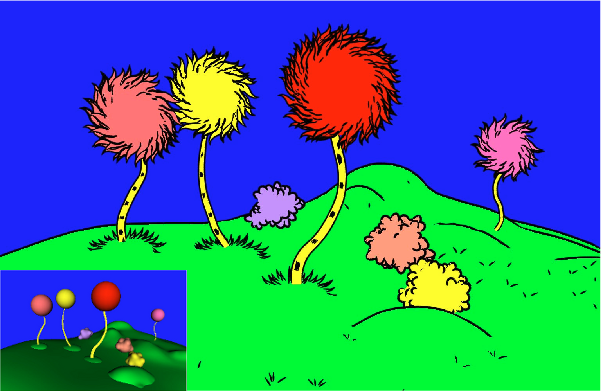
\includegraphics[width=1.0\textwidth]{img/Truffula}
\caption{A scene rendered with Kowalski-Markosian graftals, and the corresponding scene rendered with phong shading. }
\label{fig:Truffula}
\end{figure}

In the original paper, the location of the graftals was determined per-frame by first generating a “desire image” where darker areas signified higher densities of graftals, such as at the edges of the Truffula trees (See \autoref{fig:Truffula}). When a graftal is placed, it subtracts a Gaussian area (dependent on its screen-space size) from the desire image. Next, the image is searched for a desire region large enough to accommodate another graftal. This continues until no graftals can be placed. The result is a uniform distribution of graftals according to the original desire image. The authors attempted to introduce some temporal coherency by first attempting to place all of the graftals from the previous frame, but the introduction of new graftals and the removal of the old still occurred frequently enough to cause significant visual disruption.

In an extension to  their original paper, Markosian and Kowalski address the problem of temporal coherence by assigning static graftal locations to the underlying geometry, as opposed to procedurally generating them each frame \cite{Markosian2000}. They also extended the system to allow for unique methods of introducing new graftals when they are first rendered. For example, graftals can grow from a small size, rotate from behind an existing graftal, or fade in instead of simply “popping” into the scene. These improvements make this technique much more desirable for interactive scenes.

Another possible extension is animating the graftals to portray wind or other effects. Since they are completely distinct from the underlying geometry, the scene can be very easily animated, making effects such as wind very easy to implement. Additionally, since the graftal geometry can be generated on-the-fly in the geometry shader, we can create 3D graftals so that we gain subtle effects (such as parallax) as the view vector to the graftal shifts.

These techniques result in gorgeous images that effectively convey the style that they aim to recreate, but there is still much room for improvement. The largest issue is performance (the researchers report 1-5 fps for simple scenes). This research was completed in the late 90's, before programmable graphics hardware had been introduced, and has not been revisited since. Thus many of the methods discussed in the papers are quite antiquated or can be extended and optimized. For instance, much of the graftal rendering can be offloaded to the GPU. 


\subsection{Particle Systems}

A stylized rendering system using graftals is comparable to a particle system, in that graftals share much of their behavior and parameters with surface-constrained particles. One of the potential extensions discussed in the original graftal paper \cite{Markosian2000} was better distribution algorithms. In their system, Markosian et al. simply distribute the graftals manually in a preprocess. But by using a surface constrained particle system, the graftal positions can be distributed evenly (or in a directable way) over the object automatically. 

A particle system can also be used to render the graftals directly on the GPU. Basically, this system forms the base implementations upon which the graftal system is built. Latta et al. provide a great overview of GPU particle systems in their presentation from GDC ’04 \cite{Latta2004}. They detail techniques for accelerating the many integrations and CPU/GPU data transfers necessary to update the system, and how to store particle data efficiently. This paper is an oft cited resource for particle system research.

The recent presentation by Drone focuses on GPU particles that react to dynamic environments \cite{Drone2007}. She introduces many techniques for implementing particle system that takes full advantage of the GPU. Take, for instance, the “force splatting” technique in which each of the N particles in the system is rendered as a quad over the textured quad (bottom) containing the velocity information for every particle in the system. By using additive alpha blending, the force for each particle is accumulated to every other particle, taking full advantage of blending and rasterization hardware. This and other hardware friendly techniques can be applied to calculating the initial positions of surface constrained graftals.

More directly applicable to the graftal system is Drone's work pertaining to particle painting \cite{Drone2007}. This work describes how particles can leave paint splotches on objects after an interaction. First, a UV to World Space mapping is created. This is similar to the objects texture map except each texel stores world space position instead of color. This can be used to calculate positions for graftal nodes by computing their positions in a texture for each object. A system such as this would allow for dynamic positioning of such nodes. While this seems expensive to recompute each frame, if we can assume that the object’s geometry is static (as terrain or a tree would be), a UV to Model Space mapping would only need to be computed once per object. Each position would then be transformed by the object’s model matrix every frame, resulting in an inexpensive UV to World Space mapping.

Su et al. introduce a programmable particle software framework \cite{Su2005} which focuses on using surface-constrained particles to describe implicit surfaces. While most objects in real-time applications are polygonal, terrain could benefit greatly from an implicit representation. In this case, Su's paper provides methods of calculating an even distribution of graftals across the surface. One such method is Witkin-Heckbert floater particles, which are surface-constrained particles distributed to equilibrium by using a Gaussian energy function per-particle

\subsection{Rendering}
While a particle system can help to place and manage graftals, a method of stylistically rendering them is still necessary. Typically, non-photo realistic systems rely on shading effects, silhouette edge drawing, and stroke effects to convey style. In the case of a graftal-based system, graftals are used to represent strokes. 

Shading effects for a stylized scene will naturally vary by object, but traditionally a variation of "toon shading" is used. This is a technique in which the diffuse component of the lighting equation is used to access what's known as a shade map, a texture which thresholds the diffuse component to a series of discretized steps, mimicking the use of a limited color palette as in cartoons. Barla et al. introduce the idea of adding a second dimension to the shade map \cite{Barla2006}. The horizontal axis still corresponds to the shade as in the traditional 1D shade map, but the vertical axis corresponds to what Barla has dubbed “tone detail”; each step along this axis is essentially its own shade map. Thus the 2D texture can be though of as a stack of traditional 1D shade maps. An arbitrary attribute, such as depth, can be used to access the vertical dimension. In that case, as the object gets farther away, a different shade map is used to shade the object (see Figure 6). This allows for many effects such, depth-of-field, specular highlights, or level-of-abstraction (LOA).

\subsection{Silhouette Edge Rendering}
Silhouette edge rendering is an essential part of most stylized systems. Because of the reduced lighting complexity, edges are relied on to distinguish the shape of objects. In a graftal system, this is just as, if not more, important. As they are designed as an extension of the object itself, and thus share its shading, graftals rely on their edge drawing for their characterization. By using different edge rendering techniques, many distinct effects can be achieved. 

The edge buffer is a data structure that efficiently maintains a list of silhouette edges \cite{Buchanan2000}. Because graftals are made up of very few edges, this can be implemented extremely efficiently. McGuire and Hughes extend this idea by introducing the edge mesh, a geometry representation that contains per-vertex adjacency information. This allows for edge rendering to be computed entirely on the GPU \cite{McGuire2004}. Data structures such as these can make geometric edge techniques like isophote distance usable in real-time applications. Isophote distance shading relies on depth, curvature, and light direction to compute edge thickness, and produces artistic that approximate the darkened regions of a surface \cite{Goodwin2007}. Northrup and Markosian present a hybrid technique that combines the precision of geometric edges with the simplicity of image-space algorithms to produce consistent silhouette lines \cite{Northrup2000}. 


\section{Animated Film Techniques}

One advantage of pursuing a stylized rendering system is that inspiration can be taken from the domain of traditionally animated film. Because they share a common goal, to produce a series of stylized images representing a complex scene, it may be possible to adapt techniques across disciplines. Furthermore, the animation industry is much more mature, having been formed nearly a century ago, and their techniques equally so. Their contributions to the field of stylized rendering should not be ignored. Thus, an important part of this research is to attempt to identify and adapt such techniques to interactive real-time rendering.

The most common problem in adapting techniques from animated film into interactive applications is the concept of a fixed camera. In film, shots are often static (the viewpoint remains stationary), while in interactive graphics the camera is free to move in whichever way the user chooses. This often limits what can be achieved with games, since effects cannot be tailored to individual shots. For instance, in the image on the left, the grass outside of the character is represented with a static texture. This works well for the shot, but would not hold up if the camera changed position.


\begin{figure}[h]
\centering

\includegraphics[width=0.49\textwidth]{img/NarutoEdge} \hfill
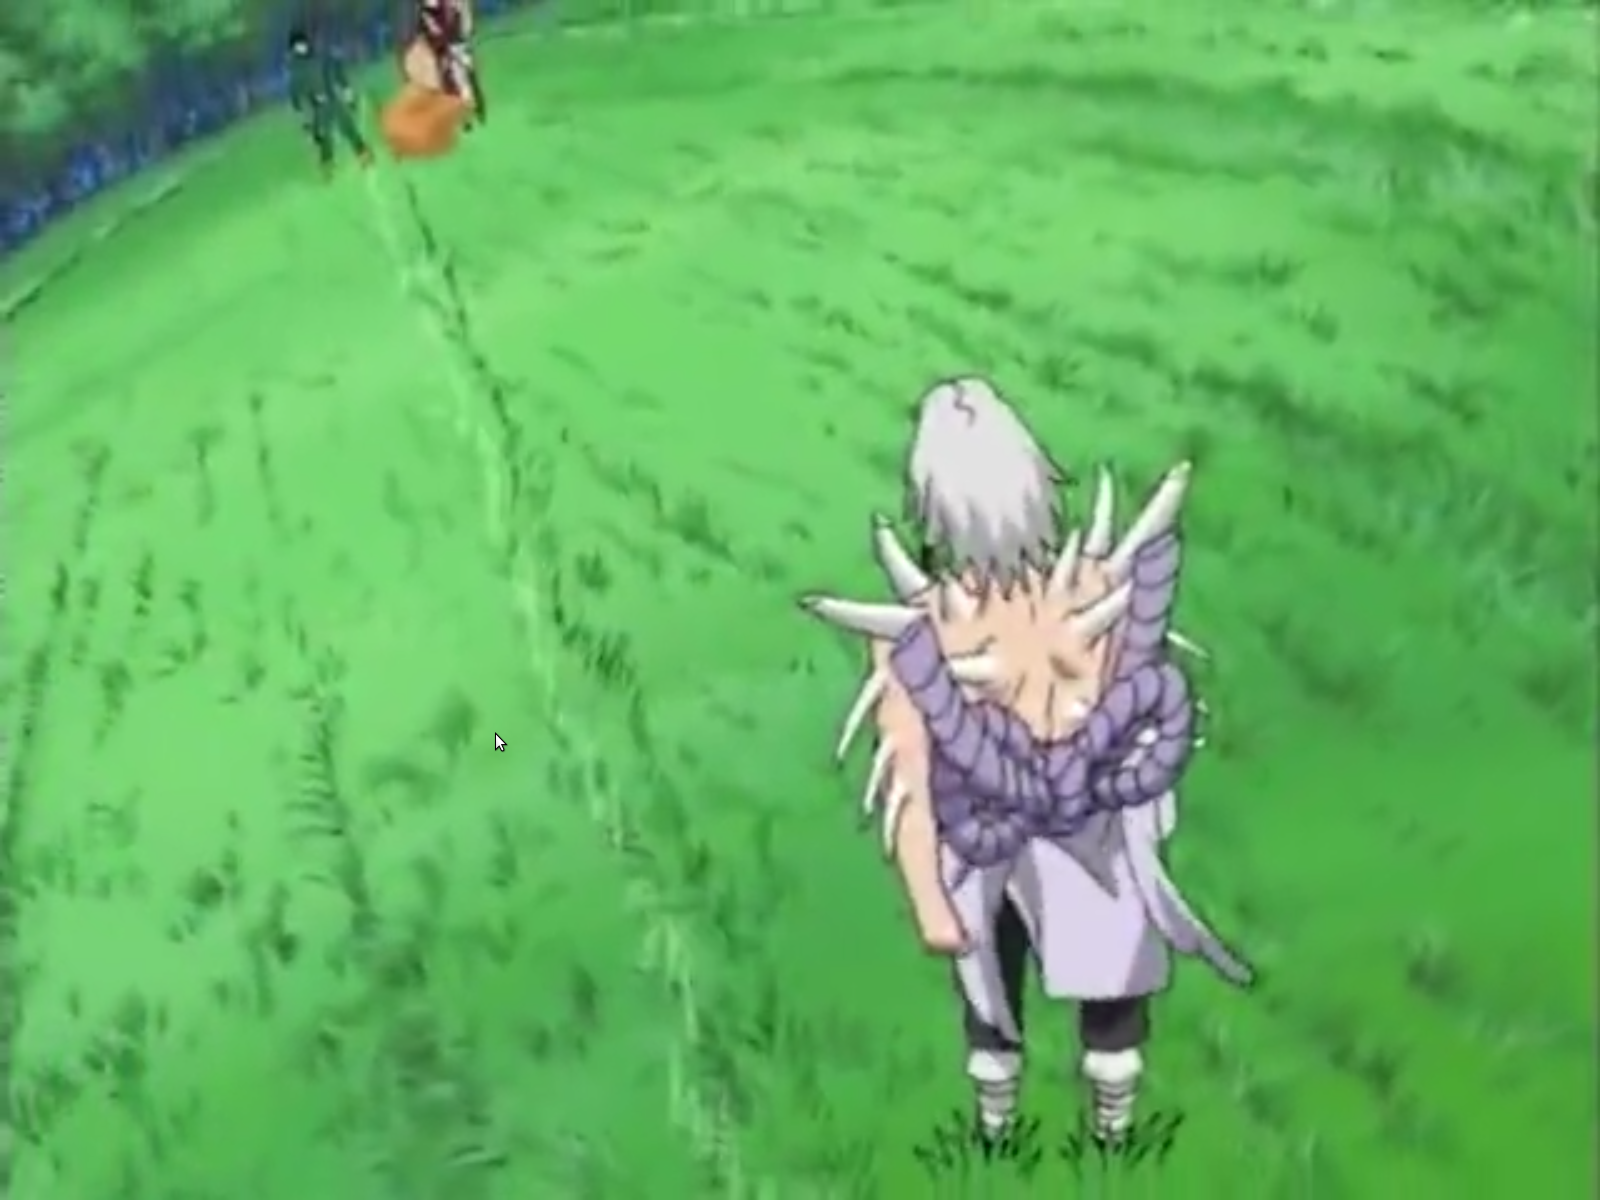
\includegraphics[width=0.49\textwidth]{img/NarutoStreak}
\caption{Two scenes from the anime \emph{Naruto}. On the left, jagged silhouettes are used to portray depth. On the right, light and dark streaks are swept across the field to represent wind-deformed grass blades.}
\label{fig:Naruto}
\end{figure}

These two scenes from the anime “Naruto” illustrate two very effective, yet simple, grass effects that can be adapted to 3D scenes (\autoref{fig:Naruto}). On the top, clever use of grass silhouettes against the character are used to portray depth. Despite the grass representation being only a simple texture, the jagged silhouettes are the only cue that the viewer needs to see depth. This observation does not entirely hold for interactive graphics; as soon as the camera is moved, the lack of parallax from the static texture breaks the illusion immediately. However, the concept behind it remains valid. The most significant area when portraying ``deep'' grass is where the grass and object intersect. By concentrating detail in that area, the viewer will make the assumption that the remaining area is just as detailed.

This is again illustrated in the bottom image, along with a technique for representing wind. The light and dark streaks in the middle of the image sweep across the field, creating the illusion of wind rustling the grass. Combined with an effect such as visible wind streaks, this could be an extremely efficient way of conveying wind for lower levels of detail since it does not rely on modifying geometry.


\bibliographystyle{plain}
\bibliography{thesis}

\end{document}
